% !TeX program = xelatex
% !TeX TXS-program:bibliography = txs:///biber

\documentclass[11pt]{article}

\usepackage[margin=1in]{geometry}
\usepackage{graphicx}
\usepackage[style=ieee,backend=biber,maxbibnames=99]{biblatex}
\usepackage{amsmath}
\usepackage{hyperref}
\usepackage{cleveref}
\usepackage{siunitx}
\usepackage{fontspec}
\usepackage{unicode-math}
%\setmainfont{TeX Gyre Pagella}
\setmathfont{Asana Math}


\addbibresource{rocpicker.bib}

\title{Finding error bands for a ROC curve}
\author{Heshy Roskes}
\date{}

\newcommand{\xdot}{\dot{x}}
\newcommand{\ydot}{\dot{y}}
\newcommand{\Xdot}{\dot{X}}
\newcommand{\Ydot}{\dot{Y}}
\newcommand{\AUC}{AUC}
\begin{document}
\maketitle

\section{Introduction}

We want to solve the following problem:

We have a set of samples characterized by a parameter \(t\) (for example, density of CD8+FoxP3+-like neighborhoods).  They are divided into two groups (responders and non-responders to anti-PD1).  We expect that one group (responders) will have a higher \(t\) than the other group (non-responders) and want to illustrate this using a ROC curve.  How can we estimate the uncertainties on the ROC curve?

One source of uncertainty is the statistics of our sample set.  We don't know the real distribution of \(t\) for the two groups; we only know the distribution for the samples we have.

Each sample's \(t\) measurement also comes with its own statistical and systematic uncertainties.  The systematic uncertainties might also be correlated between all the samples or between a subset of the samples (and this subset could include some samples from both groups).

At this point I want to address the first source of uncertainty.  I think the method will extend nicely to sample-wise uncertainties too.

\section{Previous approaches}

I haven't been able to find any recent papers that deal with this.  Many methods \autocite{roc_kerekes} deal with individual points on the ROC curve without taking their correlations into account.  There is a paper from Tilbury 25 years ago \autocite{roc_tilbury} that does something similar to what I'm doing here, but in a \emph{very} computationally expensive way, with a discrete and small number of points.  Tilbury notes that one of the computations done for that paper ``ran for over a month on a powerful Unix workstation''.  A quarter century later, I'm sure it would run faster, but the method still scales poorly with the number of points on the ROC curve.

In any case, none of the papers I saw considered any uncertainties other than the binomial statistical uncertainty on the number of samples.  We want a method that can generalize to sample-wise uncertainties, which can include statistical uncertainties on counts and any kind of systematic uncertainty.

There is something similar for Kaplan-Meier curves \autocite{kaplanmeier_sachs}.  It correctly considers the whole curve as a unit, but also doesn't include systematic uncertainties.

\section{Formalizing the problem}

A ROC curve is a plot of \(x(t), y(t)\), where \(x(t)\) is the cumulative density function (CDF) of \(t\) for one group (non-responders) and \(y(t)\) is the CDF for the other group (responders).  The derivatives, \(\xdot(t)\) and \(\ydot(t)\), give the probability density functions (PDFs) for the two groups.   We want to find a probability distribution for the ``true'' \(x\) and \(y\) distributions, given our observed data.

Our observed data for the two groups have CDFs \(X(t), Y(t)\) and PDFs \(\Xdot(t), \Ydot(t)\).  In reality, \(\Xdot\) and \(\Ydot\) are going to be sums of delta functions, while the true probability distributions \(\xdot\) and \(\ydot\) are unknown, continuous distributions.  In order to make the problem feasible, we have to make some assumptions on the form of \(\xdot\) and \(\ydot\).  The current package includes three implementations.

\subsection{Discrete points}
\label{sec:discrete}

In the first implementation, we consider \(\Xdot\) and \(\Ydot\) as discrete.  Furthermore, we assume that the true probability distributions \(\xdot\) and \(\ydot\) are also sums of delta functions, where \(\xdot\) only has nonzero probability where \(\Xdot\) does and \(\ydot\) only has nonzero probability where \(\Ydot\) does, but possibly with different relative weights.  This is equivalent to assuming that all future patients will be identical to one of the current ones.  Formally,
\begin{align}
\begin{aligned}
\Xdot(t)&=\sum_n \mathscr{X}_n \delta(t-t_n) \\
\Ydot(t)&=\sum_r \mathscr{Y}_r \delta(t-t_r) \\
\xdot(t)&=\sum_n \mathscr{x}_n \delta(t-t_n) \\
\ydot(t)&=\sum_r \mathscr{y}_r \delta(t-t_r) \\
\end{aligned}
\end{align}
The indices \(n\) and \(r\) index the non-responders and responders, \(\mathscr{X}_n\) and \(\mathscr{Y}_r\) are the numbers of non-responders and responders with \(t=t_n\) or \(t=t_r\), and \(\mathscr{x}_n\) and \(\mathscr{y}_r\) are the fractions of non-responders and responders with \(t=t_n\) or \(t=t_r\) in the true probability distribution.

\subsubsection{The most likely \texorpdfstring{\(\mathscr{x}\)}{x} and \texorpdfstring{\(\mathscr{y}\)}{y}}
\label{sec:discrete_unconstrained}

Given \(\mathscr{x}_n\) and \(\mathscr{y}_r\), the probability to observe our data \((\mathscr{X}_n, \mathscr{Y}_r)\) is
\begin{equation}
\ln{L}=-\sum_{n}\mathscr{X}_n\ln{\mathscr{x}_n}-\sum_{r}\mathscr{Y}_r\ln{\mathscr{y}_r}
\label{eq:discrete_loglikelihood}
\end{equation}
We want to maximize this likelihood with the constraint
\begin{align}
\begin{aligned}
\sum_n{\mathscr{x}_n}&=1 \\
\sum_r{\mathscr{y}_r}&=1
\end{aligned}
\label{eq:discrete_normalization}
\end{align}
We get
\begin{align}
\begin{aligned}
\frac{\partial}{\partial \mathscr{x}_n}(\ln{L} + \lambda_x \sum_n {\mathscr{x}_n} + \lambda_y \sum_r{\mathscr{y}_r})&=0 \\
-\frac{\mathscr{X}_n}{\mathscr{x}_n}+\lambda_x&=0 \\
\end{aligned}
\end{align}
The result is
\begin{align}
\begin{aligned}
\mathscr{x}_n&=\frac{\mathscr{X}_n}{\sum_{n^\prime}\mathscr{X}_{n^\prime}} \\
\mathscr{y}_r&=\frac{\mathscr{Y}_r}{\sum_{r^\prime}\mathscr{Y}_{r^\prime}}
\end{aligned}
\end{align}
In other words, the most likely probability distribution given our data is the probability distribution that we observe in the data.  No surprise.

\subsubsection{Likelihood scan for AUC}
\label{sec:discrete_likelihood_scan}

One metric that is commonly used to assess the power of \(t\) to separate the two groups is the AUC, or area under the ROC curve.  Using our notation, this is
\begin{align}
	\begin{aligned}
		\AUC&=\int_{0}^{1}ydx\\
		&=\int_{-\infty}^{\infty}y\xdot dt \label{eq:AUC}
	\end{aligned}
\end{align}
We want to find a way to estimate the error on the AUC.  To do this, we will use a likelihood scan:
\begin{enumerate}
	\item Fix the AUC to a particular value
	\item Of all possible curves \(x(t), y(t)\) that satisfy \cref{eq:AUC}, find the one that is most likely given our data
	\item Evaluate its negative log likelihood (\cref{eq:discrete_loglikelihood})
	\item Plot the best fit negative log likelihood as a function of the AUC.  The most likely AUC is the one that minimizes this log likelihood, which we found in \cref{sec:discrete_unconstrained}, and we subtract this minimum to obtain \(-2\Delta\ln{L}\).  The 68\% confidence interval is where \(-2\Delta\ln{L}<1\), and the 95\% confidence interval is where \(-2\Delta\ln{L}<3.84\).
\end{enumerate}

Our implementation uses \texttt{scipy.optimize.minimize} with \texttt{method=SLSQP}.  We introduce an explicit constraint for the AUC.  For the normalizations (\cref{eq:discrete_normalization}), we do not introduce a constraint, but instead apply the normalization internally before calculating the log-likelihood and AUC.  In our tests, this minimization converges reliably and instantaneously.

\subsection{Example}

In this simple example, we have 3 responders and 3 non-responders (in reality, there don't have to be the same number of patients in both categories).  The responders have \(t_r=(-2, -2, 1)\), while the non-responders have \(t_n=(-1, 2, 2)\).  The ROC curve is shown in \cref{fig:exampledata_discrete}.

\begin{figure}
	\begin{center}
		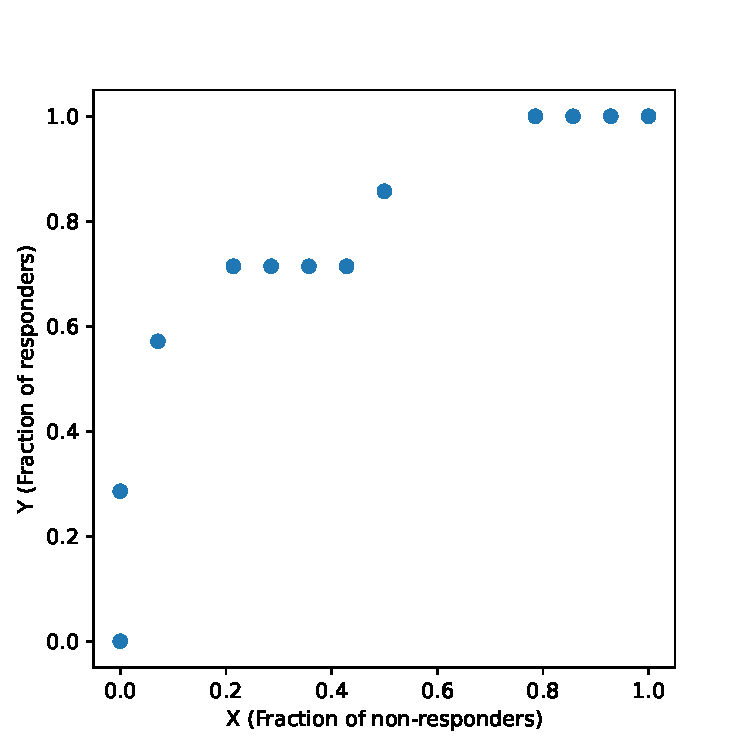
\includegraphics[width=0.32\textwidth]{discrete_exampleroc.pdf}
		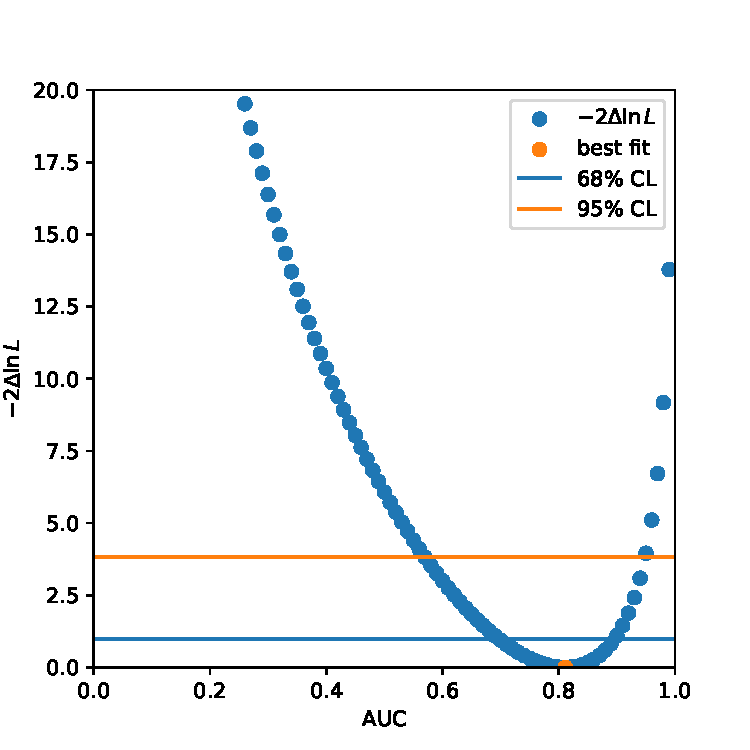
\includegraphics[width=0.32\textwidth]{discrete_scan.pdf}
		\caption{Plots for the example distributions. Left: The ROC curve. Middle: The likelihood scan. Right: The best-fitted ROC curve, with 68\% and 95\% error bands indicating the best-fitted ROC curves with AUCs at the edges of the 68\% and 95\% CL regions from the likelihood scan.}
		\label{fig:exampledata_discrete}
	\end{center}
\end{figure}

\subsection{Continuous distributions}
\label{sec:lagrangian}

In reality \(\Xdot\) and \(\Ydot\) are going to be sums of delta functions, but for the time being we will treat them as continuous and use continuous distributions in our tests.  They are normalized so that
\begin{align}
\begin{aligned}
X(-\infty)=Y(-\infty)&=0 \\
X(+\infty)&=n_X \\
Y(+\infty)&=n_Y
\end{aligned}
\end{align}

The probability density to observe a non-responder or responder at \(t_i\) is just \(\xdot(t)\) or \(\ydot(t)\), and the log likelihood is \(\ln{\xdot(t)}\) or \(\ln{\ydot(t)}\).  Summing this log likelihood over our whole observed dataset, we get
\begin{equation}
	-2\ln{L}=-2\int_{-\infty}^{\infty}dt\left(\Xdot(t)\ln{\xdot(t)}+\Ydot(t)\ln{\ydot(t)}\right).
	\label{eq:loglikelihood}
\end{equation}
We want to find \(x(t)\) and \(y(t)\), given \(\Xdot(t)\) and \(\Ydot(t)\).  Note that we have the boundary conditions
\begin{align}
\begin{aligned}
	x(-\infty)=y(-\infty)&=0\\
	x(+\infty)=y(+\infty)&=1
\end{aligned}
\label{eq:boundaryconditions}
\end{align}

To do find \(x\) and \(y\), we minimize \cref{eq:loglikelihood}.  Our Lagrangian is
\begin{equation}
	\mathcal{L}[x,\xdot,y,\ydot,t]=-2\left(\Xdot(t)\ln{\xdot(t)}+\Ydot(t)\ln{\ydot(t)}\right),
	\label{eq:lagrangian}
\end{equation}
and the Euler-Lagrange equations are
\begin{align}
\begin{aligned}
	\frac{\partial\mathcal{L}}{\partial x}-\frac{d}{dt}\frac{\partial\mathcal{L}}{\partial \xdot}&=0 \\
	-\frac{d}{dt}\left(-2\frac{\Xdot}{\xdot}\right)&=0 \\
	\frac{\Xdot}{\xdot}&=\frac{1}{A} \\
	x&=AX+B.
\end{aligned}
\end{align}
Applying the boundary conditions, and applying the symmetric logic to \(y\), we get
\begin{align}
\begin{aligned}
	x&=X/n_X \\
	y&=Y/n_Y
\end{aligned}
\end{align}
In other words, the most likely probability distribution given our data is the probability distribution that we observe in the data.  No surprise.

\subsection{Likelihood scan for AUC}

We want to produce a likelihood scan for the AUC, similar to how we did it in \cref{sec:discrete_likelihood_scan}.

To minimize the log likelihood given a fixed AUC, we add a Lagrange multiplier term to \cref{eq:lagrangian} to obtain
\begin{equation}
\mathcal{\tilde{L}}[x,\xdot,y,\ydot,t,\Lambda]=-2\left(\Xdot(t)\ln{\xdot(t)}+\Ydot(t)\ln{\ydot(t)}\right)+\Lambda y\xdot
\end{equation}
The Euler-Lagrange equations are:
\begin{align}
\begin{aligned}
\frac{\partial\mathcal{L}}{\partial x}-\frac{d}{dt}\frac{\partial\mathcal{L}}{\partial \xdot}&=0 \\
-\frac{d}{dt}\left(-2\frac{\Xdot}{\xdot}+\Lambda y\right)&=0 \\
2\frac{\Xdot}{\xdot}-\Lambda y&=c_1 \\
\Lambda y \xdot + c_1 \xdot - 2\Xdot&=0
\end{aligned}
\qquad
\begin{aligned}
\frac{\partial\mathcal{L}}{\partial y}-\frac{d}{dt}\frac{\partial\mathcal{L}}{\partial \ydot}&=0 \\
\Lambda \xdot-\frac{d}{dt}\left(-2\frac{\Ydot}{\ydot}\right)&=0 \\
2\frac{\Ydot}{\ydot}+\Lambda x&=c_2 \\
-\Lambda x \ydot + c_2 \ydot - 2\Ydot&=0 \\
\end{aligned}
\label{eq:eulerlagrange_AUC}
\end{align}

In addition to the boundary conditions from \cref{eq:boundaryconditions}, we also have \cref{eq:AUC}.  We can integrate the Euler-Lagrange equations \cref{eq:eulerlagrange_AUC} to obtain:
\begin{align}
\begin{aligned}
\int_{-\infty}^{\infty}dt\left(\Lambda y \xdot + c_1 \xdot - 2\Xdot\right)&=0 \\
\Lambda\AUC+c_1-2n_X&=0
\end{aligned}
\qquad
\begin{aligned}
\int_{-\infty}^{\infty}dt\left(-\Lambda x \ydot + c_2 \ydot - 2\Ydot\right)&=0 \\
-\Lambda(1-AUC)+c_2-2n_Y&=0
\end{aligned}
\label{eq:boundaryconditions_AUC}
\end{align}
We actually now have one boundary condition too many: we need five, one each for \(x\), \(y\), \(c_1\), \(c_2\) and \(\Lambda\).  One of them is redundant.

This system of differential equations can be solved using \texttt{scipy.integrate.solve\_bvp}.

\subsubsection{Example}

For the first example I tried a simple test with three events in each category: the non-responders have \(t=\left(-1, 2, 2\right)\) and the responders have \(t=\left(-2, -2, 1\right)\).  Instead of delta functions, the data distributions \(X(t)\) and \(Y(t)\) are sums of normal distributions with a width of \(0.6\).  The data distributions and ROC curve are shown in \cref{fig:exampledata}.

\begin{figure}
\begin{center}
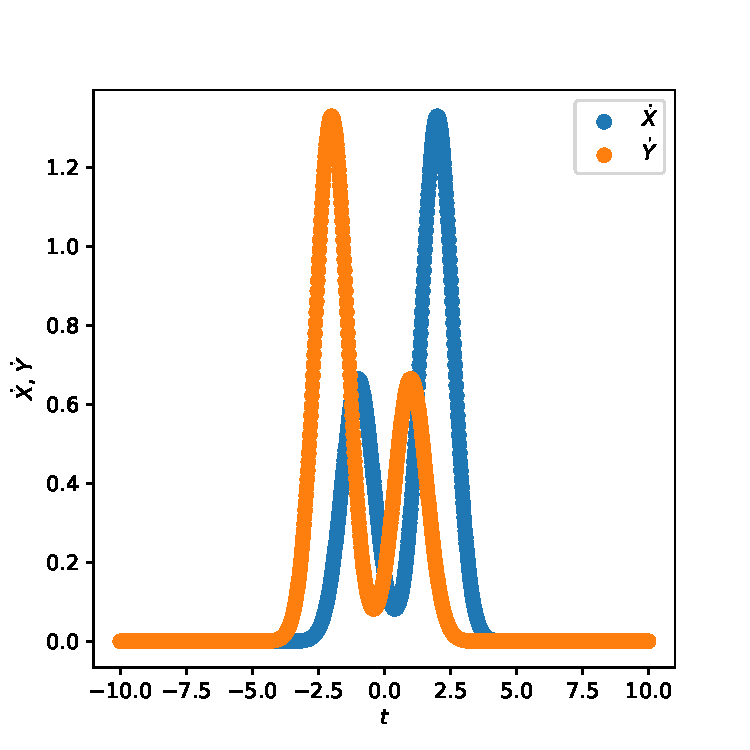
\includegraphics[width=0.32\textwidth]{exampleXdotYdot.pdf}
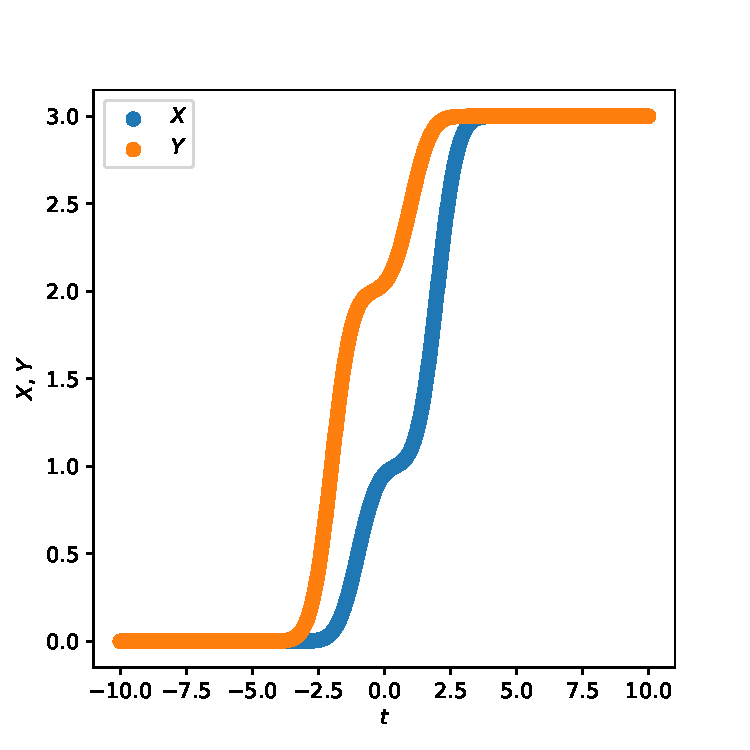
\includegraphics[width=0.32\textwidth]{exampleXY.pdf}
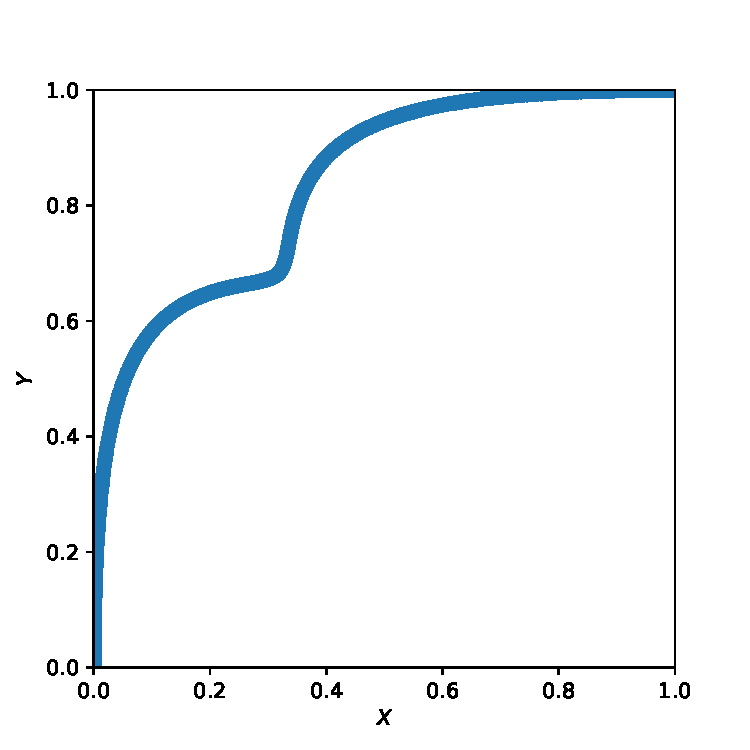
\includegraphics[width=0.32\textwidth]{exampleroc.pdf}
\caption{Plots for the example distributions.  Left: The density of non-responders \(\Xdot\) and responders \(\Ydot\).  Middle: The cumulative density of non-responders \(X\) and responders \(Y\).  Right: The ROC curve.}
\label{fig:exampledata}
\end{center}
\end{figure}

I tried plugging the differential equations \cref{eq:eulerlagrange_AUC} and boundary conditions \cref{eq:boundaryconditions,eq:boundaryconditions_AUC} into \texttt{scipy.integrate.solve\_bvp}.  For some range of \(\AUC\), this works pretty well.  I have to give it a decent starting guess for the curve and \(\Lambda\).  The way I do this is to start from the actual ROC curve (which is the solution when \(\AUC\) is the actual \(\AUC\) for \(x=X/n_X\) and \(y=Y/n_Y\)) and moving outwards in small increments.  Each time, the guess uses the fitted \(\Lambda\) and ROC curve, adjusted slightly to match the desired \(\AUC\), from the previous step.

There are two possible ways \texttt{solve\_bvp} can fail.  It can fail to converge, of course, but it can also converge on the following fake solution, which satisfies \cref{eq:eulerlagrange_AUC,eq:boundaryconditions,eq:boundaryconditions_AUC}:
\begin{align}
\begin{aligned}
x&=\Xdot/n_X \\
y&=\Ydot/n_Y \\
\Lambda&=0 \\
c_1&=2n_X \\
c_2&=2n_Y
\end{aligned}
\end{align}
In other words, \cref{eq:boundaryconditions_AUC} is a necessary but not sufficient replacement for \cref{eq:AUC}.  I'm not sure how to come up with a better boundary condition.  On the other hand, it may not matter so much, because \texttt{solve\_bvp} needs a decent guess anyway in order to converge.

A bigger issue is that beyond a certain point, \texttt{solve\_bvp} fails to converge even if I give it a guess based on an \(\AUC\) that is very close by.  A likelihood scan for \(\AUC\) in this example analysis within the range that works is shown in \cref{fig:examplelikelihoodscan}, together with the fitted values of \(\Lambda\), \(c_1\), and \(c_2\).

\begin{figure}
\begin{center}
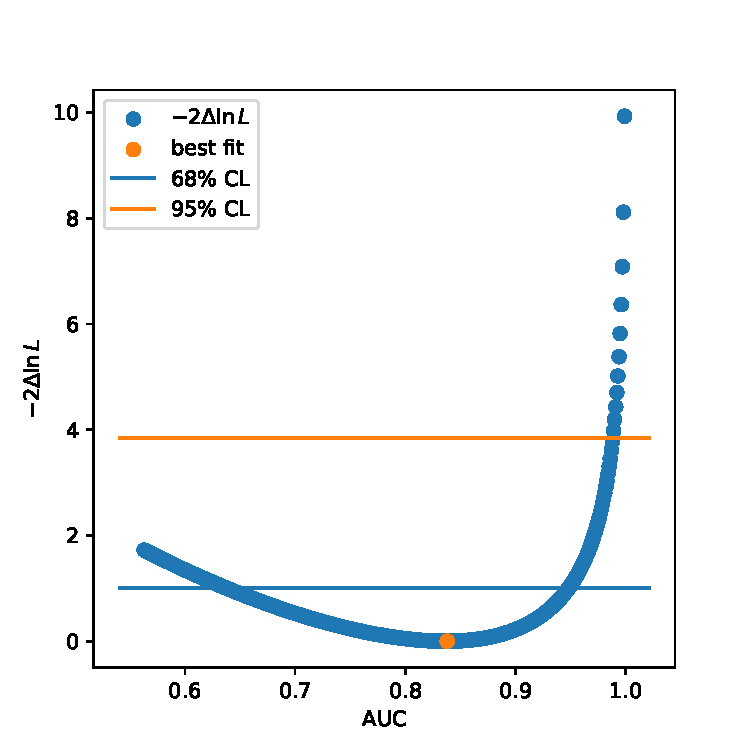
\includegraphics[width=0.32\textwidth]{examplescan.pdf}
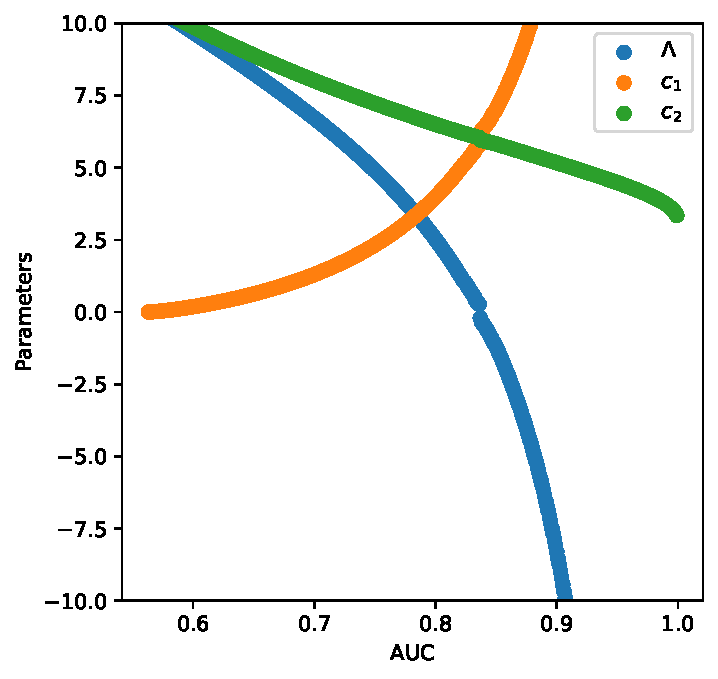
\includegraphics[width=0.32\textwidth]{exampleparameters.pdf}
\caption{Left: Likelihood scan for the \(\AUC\) using the example distributions.  Right: Fitted values of \(\Lambda\), \(c_1\), and \(c_2\) at each point in the likelihood scan.}
\label{fig:examplelikelihoodscan}
\end{center}
\end{figure}

These plots go in steps of \(\Delta\AUC=\num{0.002}\) and down to \(\AUC=\num{0.564}\); by taking successively smaller steps, I can get down to \(\AUC=\num{0.55940501}\), where \(c_1=\num{6.36e-06}\).  Either \(c_1\) asymptotically goes to 0, in which case the issue might be numerical precision and a reparameterization could help, or there is some kind of phase transition and the solution jumps somewhere else in the space of possible ROC curves and parameters.

\section{Vision for next steps}

\subsection{Treatment of \texorpdfstring{\(\Xdot\)}{X dot} and \texorpdfstring{\(\Ydot\)}{Y dot}}
\label{sec:deltafunctions}

I'm not sure yet if I should be regarding \(\Xdot\) and \(\Ydot\) as continuous, as I've been doing here, or if I should treat them as sums of \(\delta\) functions.  The issue I'm grappling with is that the real probability densities for responders and non-responders \(\xdot\) and \(\ydot\) are, of course, continuous functions.  \Cref{eq:eulerlagrange_AUC} gives \(\Xdot=0\implies\xdot=0\) and \(\Ydot=0\implies\ydot=0\), meaning that \(\xdot\) and \(\ydot\) are also \(\delta\) functions.  This is ok as far as ROC curves go, but won't work when we get a new patient (whose \(t\) will not be exactly the same as any of the previous patients) and want to predict whether they will respond to treatment.

Mathematica gives a closed-form solution to \cref{eq:eulerlagrange_AUC}.  It's in terms of integrals of \(\Xdot\) and \(\Ydot\), but if I use \(\delta\) functions I can trivially evaluate those integrals and plug in the boundary conditions to find \(c_1\), \(c_2\), and \(\Lambda\).  There might even be an analytical solution, but at the very least doing it numerically would be easier than \texttt{solve\_bvp}.

Even if I don't use \(\delta\) functions for the real result, the solution from Mathematica using them might at least give a better starting point for \texttt{solve\_bvp}.

Ideally I think I'd like to keep \(\Xdot\) and \(\Ydot\) as \(\delta\) functions (they are in data, after all) and add a term in the Lagrangian to help \(\xdot\) and \(\ydot\) to behave nicely.  The physicist in me wants this term to be \(\frac{1}{2}m(\xdot^2+\ydot^2)\), but I don't know if that's actually the right term.

Once we do this, even the unconstrained Lagrangian (\cref{eq:lagrangian}) won't minimize at \(x=X/n_X, y=Y/n_Y\), but will probably be a smoothed version of that curve.

My guess is that some of the logic underlying calculus of variations isn't technically correct when \(\Xdot\) and \(\Ydot\) are not continuous, but it will work out anyway.

\subsection{Systematics}
\label{sec:systematics}

I'll probably find mistakes in this when I go to implement it, but my preliminary feeling is that the systematics will go in the data distributions, so that \(\Xdot(t)\) and \(\Ydot(t)\) will become \(\Xdot(t,\vec{\beta})\) and \(\Ydot(t,\vec{\beta})\).  For example, let's say we have one sample at \(t=t_0\) with a log-normal systematic with a variation of \(1+\alpha\) at \(1\sigma\).  We will get
\begin{equation}
\Xdot(t,\beta)=\delta(t(1+\alpha)^\beta-t_0)
\end{equation}
and the Lagrangian will get a term
\begin{equation}
\mathcal{\tilde{L}_\beta}=\beta^2
\end{equation}

A sample will, in general, have multiple systematics, including log-normal and Poisson and probably others.  Some of the systematics will be correlated between a subset of the samples (for example flatfielding and warping will be correlated between all samples in a batch).

\subsection{Predicting response for a new patient}

Let's say we get a sample from a new patient (\(t=t^*\)) and want to predict the probability that they will respond to treatment.  I think what we want to do is to find the best fit \(\xdot\) and \(\ydot\), as described in \cref{sec:deltafunctions}, with the addition of the systematics terms described in the previous section.  Then we will evaluate \(\xdot\) and \(\ydot\) at \(t^*\).  The new sample will also have systematics, and some of them may even be correlated with the systematics of (some of) the samples in the training set.  [I imagine these correlations are mostly an issue when writing a paper, when the training and test sets might be part of the same batch, and not so much when the model is used in the clinic.  Still it's better to have the capability to get it right.]

\subsection{Kaplan-Meier curves}

I imagine that you can construct a similar Lagrangian for Kaplan-Meier curves and use a similar method to predict survival time, with appropriate uncertainties, for a new patient.

\subsection{Packaging}

My vision is to put this together in an open source package like the CMS Collaboration's Combine tool (which is about to finally get its first formal paper \autocite{CAT-23-001}).  You would input a ``datacard'', a text file that lists \(t\) and its uncertainty for each sample and response or survival time, as appropriate, and it will run the fits for you.

To continue the farming theme from CMS (Combine and its interface, Combine Harvester) I want to call it ROC Picker.  Still trying to come up with a farm-themed name for the Kaplan-Meier part.  There's a farm machinery company in Iowa called KM Ag Service$\ldots$

Nothing here is specific to IF or even imaging, so I'd put it under the AstroPath Github organization but leave it decoupled from the pipeline and database code.

\printbibliography

\end{document}